\documentclass[12pt, oneside]{book}
\usepackage[a4paper,top=2.5cm,bottom=2.5cm,left=3.5cm,right=2cm]{geometry}
\usepackage[utf8]{inputenc}
\usepackage[T1]{fontenc}
\usepackage{graphicx}
\usepackage{url}
\usepackage[slovak]{babel} % vypnite pre prace v anglictine
\usepackage{amssymb}
\usepackage{amsthm}
\usepackage{amsmath}
\usepackage{hyperref}
\usepackage{pstricks}
%\usepackage{cleveref}
\linespread{1.25} % hodnota 1.25 by mala zodpovedat 1.5 riadkovaniu
\setlength{\parskip}{1em}


\newtheorem{defn}{Definícia}
\newtheorem{lema}[defn]{Lema}
\newtheorem{veta}[defn]{Veta}
\newtheorem{dosl}[defn]{Dôsledok}
\newtheorem{pozn}[defn]{Poznámka}

% -------------------
% --- Definicia zakladnych pojmov
% --- Vyplnte podla vasho zadania
% -------------------
\def\mfrok{2018}
\def\mfnazov{Farbenia grafov s obmedzeniami do vzdialenosti dva}
\def\mftyp{Diplomová práca}
\def\mfautor{Bc. Jaroslav Petrucha}
\def\mfskolitel{RNDr. Michal Forišek, PhD.}

%ak mate konzultanta, odkomentujte aj jeho meno na titulnom liste
\def\mfkonzultant{tit. Meno Priezvisko, tit. }  

\def\mfmiesto{Bratislava, \mfrok}

%aj cislo odboru je povinne a je podla studijneho odboru autora prace
\def\mfodbor{Informatika} 
\def\program{ Informatika }
\def\mfpracovisko{ Katedra informatiky }

\begin{document}     
\frontmatter


% -------------------
% --- Obalka ------
% -------------------
\thispagestyle{empty}

\begin{center}
\sc\large
Univerzita Komenského v Bratislave\\
Fakulta matematiky, fyziky a informatiky

\vfill

{\LARGE\mfnazov}\\
\mftyp
\end{center}

\vfill

{\sc\large 
\noindent \mfrok\\
\mfautor
}

\eject % EOP i
% --- koniec obalky ----

% -------------------
% --- Titulný list
% -------------------

\thispagestyle{empty}
\noindent

\begin{center}
\sc  
\large
Univerzita Komenského v Bratislave\\
Fakulta matematiky, fyziky a informatiky

\vfill

{\LARGE\mfnazov}\\
\mftyp
\end{center}

\vfill

\noindent
\begin{tabular}{ll}
Študijný program: & \program \\
Študijný odbor: & \mfodbor \\
Školiace pracovisko: & \mfpracovisko \\
Školiteľ: & \mfskolitel \\
% Konzultant: & \mfkonzultant \\
\end{tabular}

\vfill


\noindent \mfmiesto\\
\mfautor

\eject % EOP i


% --- Koniec titulnej strany


% -------------------
% --- Zadanie z AIS
% -------------------
% v tlačenej verzii s podpismi zainteresovaných osôb.
% v elektronickej verzii sa zverejňuje zadanie bez podpisov

\newpage 
\thispagestyle{empty}
\hspace{-2cm}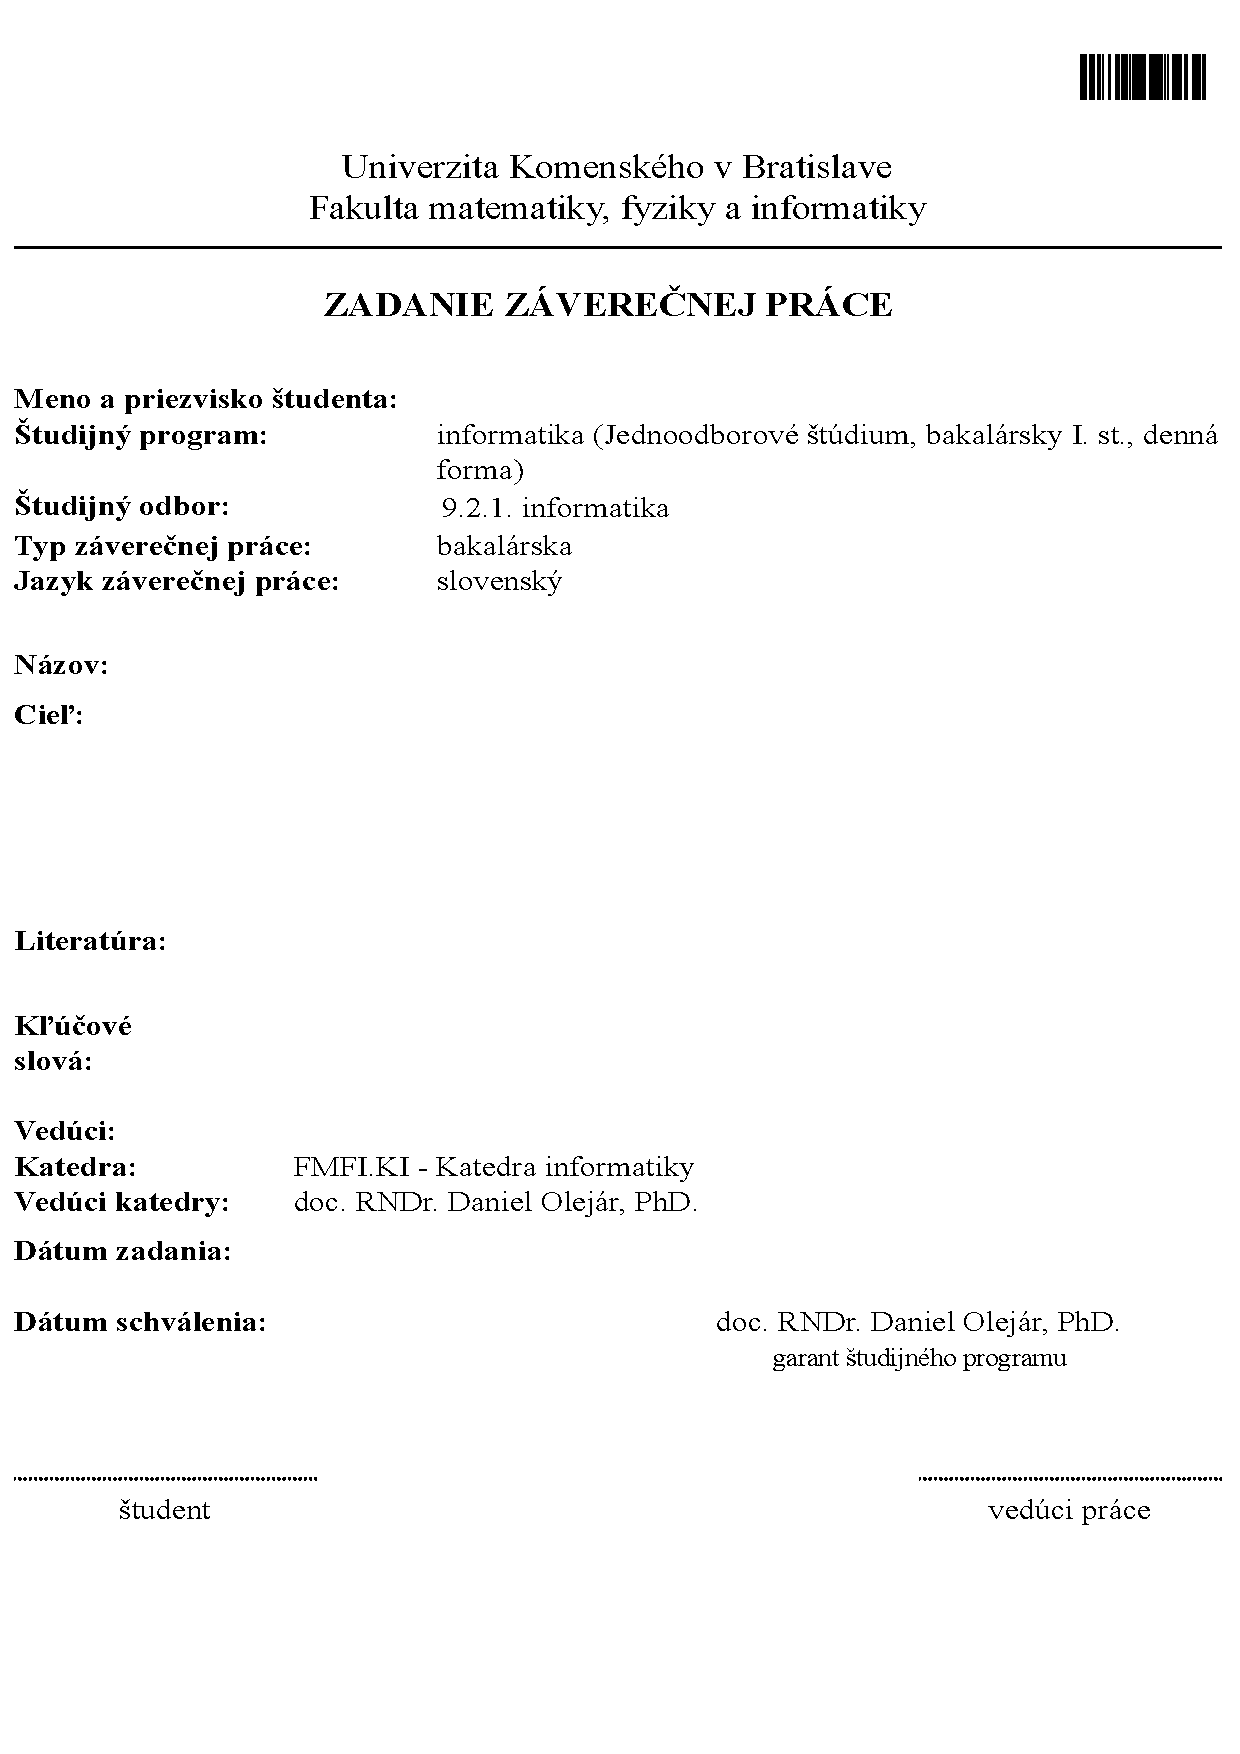
\includegraphics[width=1.1\textwidth]{images/zadanie}

% --- Koniec zadania

\frontmatter

% -------------------
%   Poďakovanie - nepovinné
% -------------------
\setcounter{page}{3}
\newpage 
~

\vfill
{\bf Poďakovanie:} Ďakujem môjmu školiteľovi, RNDr. Michalovi Foriškovi, PhD., za všetku
pomoc pri tvorbe tejto práce, či už išlo o cenné nápady k problémom, podporu pri
výskume, alebo rady k tomu, ako úspešne a načas napísať textovú podobu práce.

Ďakujem mojej rodine, ktorá ma počas celého štúdia podporovala. Ďakujem všetkým kamarátom
z Trojstenu. Ste úžasní a bez Vás by bol Matfyz chudobnejší.

V neposlednom rade ďakujem škole, jej učiteľom, docentom a profesorom, za výborných päť
rokov štúdia a veľa príležitostí rásť, najmä v smeroch, ktorými by som sa sám nevydal.

% --- Koniec poďakovania

% -------------------
%   Abstrakt - Slovensky
% -------------------
\newpage 
\section*{Abstrakt}

$L(2,1)$-farbenie grafu je očíslovanie jeho vrcholov prirodzenými číslami tak,
že čísla susedných vrcholov sa líšia aspoň o $2$ a čísla vrcholov vo vzdialenosti
$2$ sa líšia aspoň o $1$. Rozpätie $L(2,1)$ farbenia je najväčšie číslo, ktoré
používa. Minimálne rozpätie $L(2,1)$-farbenia grafu $G$ označujeme $\lambda(G)$.
Najlepší doterajší algoritmus na hľadanie $\lambda(G)$ na všeobecných grafoch má
časovú zložitosť $O^*(2.6488^n)$.

V práci popisujeme metódy rozdelenia problému na menšie časti, pomocou
ktorých vytvárame efektívnejšie algoritmy pre hľadanie $\lambda(G)$.
Vytvoríme algoritmus na hľadanie rozpätia $L(2,1)$-farbenia na planárnych
grafoch v čase $O^*(2.2^{n + o(n)})$ a v čase $O^*(2.613^n)$ na grafoch s malým
vrcholovým separátorom. Nakoniec popisujeme postup generovania všetkých neoznačených
minimálne $2$-hranovo súvislých grafov. Experimentálne overujeme, že spomedzi $2$-hranovo
súvislých grafov majú najväčší počet kombinatorickej štruktúry, ktorá sa
nazýva vlastný pár, práve kružnice.

\paragraph*{Kľúčové slová:} $L(2,1)$-farbenie, planárny graf, bezmostový graf, exponenciálny algoritmus

% --- Koniec Abstrakt - Slovensky


% -------------------
% --- Abstrakt - Anglicky 
% -------------------
\newpage 
\section*{Abstract}

$L(2,1)$-colouring of a graph is an assignment of natural numbers to its vertices such
that adjacent vertices differ by at least $2$ and vertices sharing a common neighbor
differ by at least $1$. The span of an $L(2,1)$-colouring is the largest number assigned
to a vertex. The minimum span of any $L(2,1)$-colouring of graph is denoted by $\lambda(G)$.
The best current algorithm for determining $\lambda(G)$ for general graphs has
time complexity of $O^*(2.6488^n)$.

We describe methods for splitting the problem into independent smaller parts
and use them to develop faster algorithms for determining $\lambda(G)$.
We showcase our method for the planar graphs, for which we create an $O^*(2.2^{n + o(n)})$
algorithm. We create an algorithm for graphs with small cuts having time complexity
$O^*(2.613^n)$. Last, we develop an algorithm for generating all the minimally $2$-edge-connected
graphs. Using this, we experimentally verify that cycles have the most proper pairs from
the class of $2$-edge-connected graphs.

\paragraph*{Keywords:} $L(2,1)$-colouring, planar graph, edge-free graph, exponential-time algorithm 

% --- Koniec Abstrakt - Anglicky

% -------------------
% --- Predhovor - v informatike sa zvacsa nepouziva
% -------------------
%\newpage 
%\thispagestyle{empty}
%
%\huge{Predhovor}
%\normalsize
%\newline
%Predhovor je všeobecná informácia o práci, obsahuje hlavnú charakteristiku práce 
%a okolnosti jej vzniku. Autor zdôvodní výber témy, stručne informuje o cieľoch 
%a význame práce, spomenie domáci a zahraničný kontext, komu je práca určená, 
%použité metódy, stav poznania; autor stručne charakterizuje svoj prístup a svoje 
%hľadisko. 
%
% --- Koniec Predhovor


% -------------------
% --- Obsah
% -------------------

\newpage 

\tableofcontents

% ---  Koniec Obsahu

% -------------------
% --- Zoznamy tabuliek, obrázkov - nepovinne
% -------------------

\newpage 

\listoffigures
%\listoftables

% ---  Koniec Zoznamov

\mainmatter


\input uvod.tex 

\input zaklady.tex

\input osekavanie.tex

\input ciastfarbenia.tex

\input hranovosuvisle.tex

\input zaver.tex

% -------------------
% --- Bibliografia
% -------------------


\newpage	

\backmatter

\thispagestyle{empty}
\nocite{*}
\clearpage

\bibliographystyle{plain}
\bibliography{literatura} 

%Prípadne môžete napísať literatúru priamo tu
%\begin{thebibliography}{5}
 
%\bibitem{br1} MOLINA H. G. - ULLMAN J. D. - WIDOM J., 2002, Database Systems, Upper Saddle River : Prentice-Hall, 2002, 1119 s., Pearson International edition, 0-13-098043-9

%\bibitem{br2} MOLINA H. G. - ULLMAN J. D. - WIDOM J., 2000 , Databasse System implementation, New Jersey : Prentice-Hall, 2000, 653s., ???

%\bibitem{br3} ULLMAN J. D. - WIDOM J., 1997, A First Course in Database Systems, New Jersey : Prentice-Hall, 1997, 470s., 

%\bibitem{br4} PREFUSE, 2007, The Prefuse visualization toolkit,  [online] Dostupné na internete: <http://prefuse.org/>

%\bibitem{br5} PREFUSE Forum, Sourceforge - Prefuse Forum,  [online] Dostupné na internete: <http://sourceforge.net/projects/prefuse/>

%\end{thebibliography}

%---koniec Referencii

% -------------------
%--- Prilohy---
% -------------------

%Nepovinná časť prílohy obsahuje materiály, ktoré neboli zaradené priamo  do textu. Každá príloha sa začína na novej strane.
%Zoznam príloh je súčasťou obsahu.
%
%\addcontentsline{toc}{chapter}{Appendix A}
%\input AppendixA.tex
%
%\addcontentsline{toc}{chapter}{Appendix B}
%\input AppendixB.tex

\end{document}






